\section{Методы получения нижних и верхних оценок}

\subsection{Fooling Set}

Пусть дана матрица некоторой функции. Выберем клетки этой таблицы $a_1, a_2, \ldots, a_n$ так, чтобы
никакие две из них не могли оказаться в одном <<одноцветном>> прямоугольнике, то есть состоящего только
из нулей или только из единиц. Тогда для каждой клетки должен быть свой прямоугольник разбиения. Отсюда
следует, что в дереве протокола должно быть хотя бы $n$ вершин, а высота дерева хотя бы $\log n$. Этот
метод называется \deftext{Fooling Set}.  

Например, его можно применить для функции
$$
    \EQ(x, y) \coloneqq
    \begin{cases}
        1, & x = y,\\
        0, & x \neq y,
    \end{cases}
$$
на строчках длины $m$ мы получим диагональную матрицу $2^m \times 2^m$, и тогда в качестве точек $a_i$
можно выбрать единицы на диагональной матрице. Понятно, что никакие две из них не находятся в одном
одноцветном прямоугольнике. Значит высота коммуникационного дерева хотя бы $\log 2^m = m$.

Похожим образом мы можем доказать нижнюю оценку на функцию $\Disj(x, y)$ на подмножествах множества
$[n]$, которая принимает значение $1$ тогда и только тогда, когда $ x \cap y = \emptyset$. Для всех
множеств $S \in [2^n]$ рассмотрим ячейку матрицы $a_S \coloneqq (S, \overline{S}$). Заметим, что для $S
\neq S'$ ячейки $a_S$ и $a_{S'}$ не могут лежать в одном прямоугольнике, так как иначе в этом
прямоугольнике лежат ячейки $(S, \overline{S'})$, $(S', \overline{S})$, и в одной из них стоит $0$. Из
чего мы можем заключить, что высота коммуникационного дерева хотя бы $\log 2^n = n$.  


\subsection{Rectangle Size}

Коммуникационную сложность можно несложно оценить через размеры одноцветных прямоугольников в покрытии
коммуникационной матрицы.


\begin{lemma}[Rectangle Size]
    Пусть $S \subseteq X \times Y \times O$ некоторое отношение и размер любого одноцветного
    прямоугольника имеет долю не больше $\varepsilon$ от размера всего $M_S$. Тогда $\chi \ge
    \frac{1}{\varepsilon}$.

    В частности, $\DCC(S) \ge \log \frac{1}{\varepsilon}$.
\end{lemma}

\begin{remark}
    Бывает полезно рассматривать покрытие не всей матрицы, а только какого-то из цветов в отдельности.
\end{remark}

$\IP(x, y) = \sum x_iy_i \bmod 2$.

\begin{theorem}
    $\DCC(\IP) = n + 1$.
\end{theorem}

\begin{proof}
    Покажем, что любой одноцветный прямоугольник имеет площадь не более $2^n$. Тогда прямоугольников хотя
    бы $2^n$.

    Пусть $R = A \times B$ и имеет цвет $c$. Пусть $\dim A = k$, и пусть $A$ лежит в линейной оболочке
    $\avg{a_1, a_2, \dots, a_k}$, где все $a_i \in A$. Заметим, что $|A| \le 2^k$. Все элементы $b \in B$
    удовлетворяют линейной системе $\IP(a_i, b) = c$ для всех $i \in [k]$. У такой системы не более
    $2^{n - k}$ решений, поэтому $|B| \le 2^{n - k}$.
\end{proof}

Мы уже доказывали, что $\DCC(\Disj) \ge n + 1$. Докажем ещё раз (правда, с худшей константой), используя
технику Rectangle Size.

\begin{theorem}
    $\DCC(\Disj) = \Omega(n)$.
\end{theorem}

\begin{proof}
    Посмотрим только на клетки, у которых $\Disj(x, y) = 1$. Их $3^n$ (каждый бит принадлежит либо $x$,
    либо $y$, либо не принадлежит обоим).

    Теперь посмотрим на $1$-прямоугольник $A \times B$. Для всех $a \in A, b \in B$ выполнено $a \cap
    b = \emptyset$, следовательно $A' \coloneqq \bigcup\limits_{a \in A} a$ не пересекается с
    $B' \coloneqq \bigcup\limits_{b \in B} b$. Тогда $|A'| + |B'| \le n$. Заметим, что $|A| \le 2^{|A'|}$
    (все подмножества $A'$), $|B| \le 2^{|B'|}$. Таким образом, $|A||B| \le 2^{|A'| + |B'|} \le 2^n$.

    Следовательно, прямоугольников хотя бы $\frac{3^n}{2^n} = 1.5^n$. Тогда $\DCC(\Disj) \ge
    n \log_2 (1.5) = \Omega(n)$.
\end{proof}

Вместо размеров прямоугольников можно рассматривать произвольную меру.

\begin{lemma}[Rectangle Measure]
    Пусть $S \subseteq X \times Y \times O$ некоторое отношение и мера $\mu$ любого одноцветного
    прямоугольника имеет долю не больше $\varepsilon$ от размера всего $M_S$. Тогда $\chi \ge
    \frac{1}{\varepsilon}$.

    В частности, $\DCC(S) \ge \log \frac{1}{\varepsilon}$.
\end{lemma}

\begin{remark}
    Меру всего множества (всех клеток $M_f$ или всех клеток какого-то цвета) обычно выбираем равной
    единице.
    
    Здесь тоже бывает полезно рассматривать покрытие не всей матрицы, а только какого-то из цветов в
    отдельности.
\end{remark}

Заметим, что Fooling Set не сильнее данной техники. Если $S$~--- Fooling Set, то введём $\mu(x, y) =
\frac{\One_{(x, y) \in S}}{|S|}$.


\subsection{Fooling Set для случайных функций}

Оценим, насколько хорош Fooling Set <<в целом>>.

Будем рассматривать случайные функции $f\colon \{0, 1\}^n \times \{0, 1\}^n \to \{0, 1\}$, где каждая
клетка $M_f$ заполняется случайно и независимо.

\begin{theorem}
    Для случайной функции с высокой вероятностью $\DCC(f) \ge \Omega(n)$.
\end{theorem}

\begin{proof}
    Всего функций такого вида $2^{2^{2n}}$.

    Протоколов с $\ell$ листьями:
    \begin{itemize}
        \item $2^{\ell}$~--- ответ в каждом листе;
        \item $(2^{2^n + 1})^{\ell}$~--- чей ход и функция игрока в каждой внутренней вершине (их $\ell -
            1$);
        \item число упорядоченных бинарных деревьев с $\ell$ листьями не больше числа Каталана $C_{\ell -
            1} \le 2^{2\ell}$ (но нас устроит и, например, оценка $C_{2\ell}$).
    \end{itemize}
    Итого получаем, что протоколов не более $2^{(2^n + 4) \ell}$.
    
    Значит, для почти всех функций (т. е. с высокой вероятностью) выполняется $\ell \ge c 2^n$. Тогда
    $\DCC(f) \ge cn$ с высокой вероятностью. То есть почти все функции~--- <<сложные>>. 
\end{proof}


\begin{theorem}
    С большой вероятностью максимальный Fooling Set случайной функции имеет размер $\bigO(\log n)$.
\end{theorem}

\begin{proof}
    Оценим вероятность, что для случайной функции найдётся Fooling Set размера $t$.

    Это должен быть комбинаторный квадрат с одноцветной диагональю (вероятность $2 \cdot 2^{-t}$), и для
    каждой из $t(t - 1) / 2$ пар клеток диагонали хотя бы в одном из углов образовываемого прямоугольника
    должен быть другой цвет (вероятность $(3 / 4)^{t(t - 1) / 2}$). Способов выбрать $t$ клеток в
    качестве диагональных не больше $\binom{n^2}{t} \le n^{2t}$. Тогда с высокой вероятностью $t \le
    \bigO{\log n}$. 
\end{proof}

Получается, Fooling Set даёт нижнюю оценку на коммуникационную сложность случайной функции не лучше
$\Omega(\log\log n)$. А реальная сложность $\Omega(n)$.


\subsection{Rank Technique}

Рассмотрим еще одну технику получения нижних оценок.

\begin{remark}
    $\rk(A + B) \le \rk(A) + \rk(B)$
\end{remark}

Пусть $\{R_i\}$~--- набор $1$-прямоугольников разбиения матрицы $M_f$, их $\chi_1(f)$ штук. Обозначим за
$\One_{R_i}$ матрицу размерности как $M_f$, в которой единицы только на месте прямоугольника $R_i$. Тогда
$M_f = \sum\limits_{i} \One_{R_i}$, но $\rk_{\field}(M_f) \le \sum \rk_{\field}(\One_{R_i}) = \chi_1$ для
любого поля $\field$, так как ранг $1$-прямоугольника равен единице.

Выберем поле $\mathbb{R}$, чтобы $\rk$ был побольше.


\begin{theorem}
    $\chi_1 \ge \rk_{\mathbb{R}}(M_f)$. Более того, $\DCC(f) \ge \log (2 \rk_{\mathbb{R}}(M_f) - 1)$.
\end{theorem}


\begin{proof}
    Первую часть уже доказали.

    Заметим, что $\rk(\overline{M_f}) \le \chi_0$ (аналогично доказанному неравенству). Кроме того,
    $\rk(M_f + \overline{M_f}) = \One$, поэтому их ранги отличаются не более, чем на единицу: $\rk(M_f)
    \le \One + \rk(-\overline{M_f}) = 1 + \rk(\overline{M_f})$, аналогично в другую сторону.

    Тогда $2\rk(M_f) - 1 \le \rk(M_f) + \rk(\overline{M_f}) \le \chi_0 + \chi_1 = \chi$, а $\DCC(f) \ge
    \log \chi$.
\end{proof}

\begin{theorem}
    $\DCC(f) \le \rk_{\field_2}(M_f) + 1 \le \rk_{\mathbb{R}}(M_f) + 1$.
\end{theorem}

\begin{proof}
    $M_f = \sum\limits^{\rk(M_f)}_{i = 1} M_i$, где $M_i$~--- матрицы ранга 1. Каждая строка такой
    матрицы $M_i$ либо $v_i$, либо $\vec 0$. Тогда Алиса для каждой матрицы $M_i$ посылает тип строки
    $x$: $\vec 0$ или $v_i$ (то есть по биту на каждую $M_i$).

    Боб складывает $v_i$ для тех матриц, в которых у Алисы $v_i$ (а не $\vec 0$), и получает строку,
    совпадающую со строкой $(M_f)_x$. В этой строке он смотрит на бит в позиции $y$~--- это и будет
    ответ. Итого переслано $\rk(M_f) + 1$ бит. 
\end{proof}

\begin{theorem}[Lovett \cite{Lovett16-root}]
    $\DCC(f) \le \polylog(\rk_{\mathbb{R}}(M_f)) \sqrt{\rk_{\mathbb{R}}(M_f)}$
\end{theorem}

Доказывать не будем. План: если ранг маленький, тогда есть большой одноцветный прямоугольник, с помощью
него уменьшим размер задачи, рекурсивно спустимся.

Давно открытая проблема~--- log-rank conjecture: $\DCC(f) \le \polylog(\rk_{\mathbb{R}}(M_f))$? Известно,
что для $\log$ вместо $\polylog$ утверждение неверно: есть пример со степенью логарифма $\approx 1.4$ или
что-то вроде.

\subsubsection{Оценки рангов матриц \texorpdfstring{$\IP$}{IP} и \texorpdfstring{$\Disj$}{DISJ}}

\begin{theorem}
    \label{th:rk(IP)-lower-bound}
    $\rk_{\mathbb{R}}(M_{\IP}) \ge 2^n - 1$.
\end{theorem}

\begin{proof}
    $\rk(AB) \le \min(\rk(A), \rk(B))$, поэтому если докажем нижнюю оценку на ранг $M^2$, то и для $M$
    докажем.

    \paragraph{Доказательство с лекции.}
    На диагонали $M^2$: в клетке $(x, x)$ при $x \neq 0$ стоит $\sum\limits_y\avg{x, y} \avg{y, x} =
    \sum\limits_y \avg{x, y}^2$. Сколько единичных слагаемых получится? У нас одно линейное уравнение над
    $\field_2$, поэтому $2^{n - 1}$. Так что на диагонали везде $2^{n - 1}$, кроме $(0, 0)$.

    Не на диагонали $M^2$: в клетке $(x, z)$ при ненулевых различных $x$ и $z$ стоит $\sum\limits_y
    \avg{x, y} \avg{y, z}$. Сколько единичных слагаемых? $x$ и $z$ линейно независимы, поэтому ранг
    системы равен $2$, поэтому решений $2^{n - 2}$.

    В строчке $0$ и столбце $0$ все значения равны нулю.

    Ранг такой матрицы не меньше $2^n - 2$: это диагональная матрица (но с одним нулём на диагонали) плюс
    матрица из одинаковых чисел.
    %\mycomment{Можно ли отсюда получить оценку $\ge 2^n - 1$, мне неочевидно. На консультации было
    %предложено другое доказательство.}

    \paragraph{Доказательство с консультации.}
    Перейдём к $\pm 1$-матрице: $M'_{x, y} = (-1)^{\avg{x, y}}$. Заметим, что $M' = \One - 2M$. Если мы
    покажем, что ранг $M'^2$ равен $2^n$, тогда ранг $M'$ равен $2^n$, тогда $M$ имеет ранг не меньше
    $2^n - 1$.

    $M'^2_{x, z} = \sum\limits_y (-1)^{\avg{x, y}} (-1)^{\avg{y, z}} =
    \sum\limits_y (-1)^{\avg{y, x + z}}$. Если $x = z$, то $x + z = 0$, то есть сумма равна $2^n$~--- это
    числа на диагонали $M'^2$. Если $x \neq z$, то ровно половина $y$ будет давать произведение $1$, а
    другая половина~--- $0$, поэтому сумма получится равной $0$.

    Получили, что матрица $M'^2$ "--- диагональная, причём все элементы на диагонали не нули. Значит, она
    имеет ранг $2^n$.
\end{proof}

\begin{theorem}
    $\rk(M_{\Disj}) = 2^n$, то есть $M_{\Disj}$ имеет полный ранг.
\end{theorem}

\begin{proof}
    Обозначим $M_n = M_{\Disj_n}$. Заметим, что $M_n = M_{n - 1} \otimes M_1$ (тензорное произведение),
    тогда $M_n = M^{\otimes n}_1$. Известно, что $\rk(A \otimes B) = \rk(A) \rk(B)$. $\rk(M_1) = 2$,
    поэтому $\rk(M_n) = 2^n$. 
\end{proof}

Матрицы с большим rigidity~--- меняем мало элементов, ранг всё равно остаётся большим. Явное построение
таких матриц~--- открытый вопрос. Они дают сложные функции для схем и другие важные
последствия. Случайные матрицы удовлетворяют этому свойству.

\subsubsection{Ранг матрицы случайной функции}
Мы уже знаем, что сложность случайных функций почти всегда большая. Будет ли большим ранг матрицы?

\begin{theorem}
    С константной вероятностью $\field_2$-ранг случайной $\{0, 1\}$-матрицы $n \times n$ будет полным.
\end{theorem}

\begin{proof}
    Выбираем каждую новую строку так, чтобы не попасть в оболочку предыдущих. Вероятность успеха:
    $p = (1 - 2^{-n}) (1 - 2^{-n + 1}) \dots (1 - 2^{-n + (n - 1)})$. Воспользуемся тем, что $\log_2(1 -
    x) \ge -2x$ для $x \le 1 / 2$:
    $$
        \log p = \sum\limits_{i = 0}^{n - 1} \log(1-2^{-n+i}) \ge
        -2\sum\limits_{i = 0}^{n - 1} 2^{-n + i} \ge -2.
    $$
    Так что $p \ge 1 / 4$.
\end{proof}

\subsubsection{Fooling Set\texorpdfstring{$\implies$}{ => }Rank Technique}

\begin{theorem}
    Пусть есть Fooling Set размера $k$. Тогда для любого поля $\field$ выполняется $\rk_\field(M_f) \ge
    \sqrt{k} - 1$.
\end{theorem}

\begin{proof}
    Пусть $S$~--- Fooling Set, причём на диагонали у него единички (если нули, перейдём к
    $\overline{M_f}$~--- отсюда появится <<$-1$>> в оценке). $S$ образует комбинаторный квадрат, назовём
    его $M'$.

    $A \odot B$~--- покоординатное умножение матриц. $A \odot B$ является подматрицей $A \otimes B$,
    поэтому $\rk(A \odot B) \le \rk(A) \cdot \rk(B)$.

    Заметим, что $M' \odot M'^T = E_{|S|}$. Тогда $|S| = \rk(E_{|S|}) \le \rk(M')^2 \le \rk(M_f)^2$.
\end{proof}

\begin{corollary}
    Для $\IP$ размер Fooling Set не больше $(n + 1)^2$.
\end{corollary}

\begin{proof}
    В поле $\field_2$ выполняется $M_{\IP} = X \times Y^T$, поэтому $\rk_{\field_2} M_{\IP} \le
    n$. Применяя только что доказанную теорему, получаем требуемое.
\end{proof}

Таким образом мы ситуацию с техниками мы можем изобразить на рисунке \ref{fig:techniques-and-functions}.
\begin{figure}[h]
    \centering
    \tikzset{
    curve-technique/.pic = {
        \fill[#1, opacity = 0.3] (-2, 0) arc (180:360:2) to[out = 90, in = 0] (0, 4) to[out = 180, in = 90] (-2, 0) -- cycle;
        \draw[#1!80, thick] (-2, 0) arc (180:360:2) to[out = 90, in = 0] (0, 4) to[out = 180, in = 90] (-2, 0) -- cycle;
    }
}
    

    
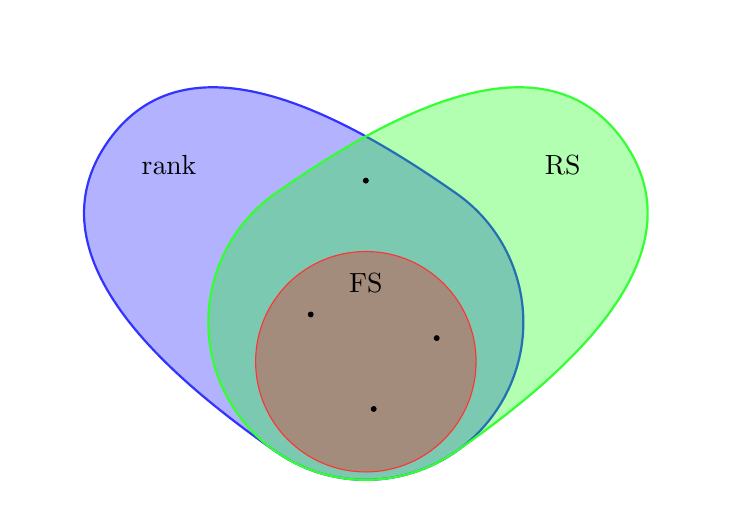
\begin{tikzpicture}[>=latex]
    \pic[rotate = 55] {curve-technique = {blue}};
    \pic[rotate = -55] {curve-technique = {green}};

    \fill[red, opacity = 0.3] (0, -0.5) circle (1.4);
    \draw[red!80] (0, -0.5) circle (1.4);

    \node at (0, 0.5) {FS};
    \node at (-2.5, 2) {rank};
    \node at (2.5, 2) {RS};

    \draw[fill = black] (-0.7, 0.1) circle (0.03) node[below] {$\EQ$};
    \draw[fill = black] (0.9, -0.2) circle (0.03) node[below] {$\GT$};
    \draw[fill = black] (0.1, -1.1) circle (0.03) node[below] {$\Disj$};

    \draw[fill = black] (0, 1.8) circle (0.03) node[below] {$\IP$};
\end{tikzpicture}
    \caption{Техники и оценки}
    \label{fig:techniques-and-functions}
\end{figure}